\documentclass{article}

\usepackage{fancyhdr}
\usepackage{extramarks}
\usepackage{amsmath}
\usepackage{amsthm}
\usepackage{amsfonts}
\usepackage{tikz}
\usepackage[plain]{algorithm}
\usepackage{algpseudocode}

\usetikzlibrary{automata,positioning}

%
% Basic Document Settings
%

\topmargin=-0.45in
\evensidemargin=0in
\oddsidemargin=0in
\textwidth=6.5in
\textheight=9.0in
\headsep=0.25in

\linespread{1.1}

\pagestyle{fancy}
\lhead{\hmwkAuthorName}
\chead{\hmwkClass\ (\hmwkClassInstructor\ \hmwkClassTime): \hmwkTitle}
\rhead{\firstxmark}
\lfoot{\lastxmark}
\cfoot{\thepage}

\renewcommand\headrulewidth{0.4pt}
\renewcommand\footrulewidth{0.4pt}

\setlength\parindent{0pt}

%
% Create Problem Sections
%

\newcommand{\enterProblemHeader}[1]{
    \nobreak\extramarks{}{Problem \arabic{#1} continued on next page\ldots}\nobreak{}
    \nobreak\extramarks{Problem \arabic{#1} (continued)}{Problem \arabic{#1} continued on next page\ldots}\nobreak{}
}

\newcommand{\exitProblemHeader}[1]{
    \nobreak\extramarks{Problem \arabic{#1} (continued)}{Problem \arabic{#1} continued on next page\ldots}\nobreak{}
    \stepcounter{#1}
    \nobreak\extramarks{Problem \arabic{#1}}{}\nobreak{}
}

\setcounter{secnumdepth}{0}
\newcounter{partCounter}
\newcounter{homeworkProblemCounter}
\setcounter{homeworkProblemCounter}{1}
\nobreak\extramarks{Problem \arabic{homeworkProblemCounter}}{}\nobreak{}

%
% Homework Problem Environment
%
% This environment takes an optional argument. When given, it will adjust the
% problem counter. This is useful for when the problems given for your
% assignment aren't sequential. See the last 3 problems of this template for an
% example.
%
\newenvironment{homeworkProblem}[1][-1]{
    \ifnum#1>0
        \setcounter{homeworkProblemCounter}{#1}
    \fi
    \section{Problem \arabic{homeworkProblemCounter}}
    \setcounter{partCounter}{1}
    \enterProblemHeader{homeworkProblemCounter}
}{
    \exitProblemHeader{homeworkProblemCounter}
}

%
% Homework Details
%   - Title
%   - Due date
%   - Class
%   - Section/Time
%   - Instructor
%   - Author
%

\newcommand{\hmwkTitle}{Homework\ \#1}
\newcommand{\hmwkDueDate}{January 24, 2020}
\newcommand{\hmwkClass}{Physics 216}
\newcommand{\hmwkClassTime}{Section 509}
\newcommand{\hmwkClassInstructor}{Dr. Ostrovskaya}
\newcommand{\hmwkAuthorName}{\textbf{Amari West}}
\newcommand{\hmwkDueTime}{11:59pm (Pages 11)}

%
% Title Page
%

\title{
    \vspace{2in}
    \textmd{\textbf{\hmwkClass:\ \hmwkTitle}}\\
    \normalsize\vspace{0.1in}\small{Due\ on\ \hmwkDueDate\ at \hmwkDueTime}\\
    \vspace{0.1in}\large{\textit{\hmwkClassInstructor\ \hmwkClassTime}}
    \vspace{3in}
}

\author{\hmwkAuthorName}
\date{}

\renewcommand{\part}[1]{\textbf{\large Part \Alph{partCounter}}\stepcounter{partCounter}\\}

%
% Various Helper Commands
%

% Useful for algorithms
\newcommand{\alg}[1]{\textsc{\bfseries \footnotesize #1}}

% For derivatives
\newcommand{\deriv}[1]{\frac{\mathrm{d}}{\mathrm{d}x} (#1)}

% For partial derivatives
\newcommand{\pderiv}[2]{\frac{\partial}{\partial #1} (#2)}

% Integral dx
\newcommand{\dx}{\mathrm{d}x}

% Alias for the Solution section header
\newcommand{\solution}{\textbf{\large Solution}}

% Probability commands: Expectation, Variance, Covariance, Bias
\newcommand{\E}{\mathrm{E}}
\newcommand{\Var}{\mathrm{Var}}
\newcommand{\Cov}{\mathrm{Cov}}
\newcommand{\Bias}{\mathrm{Bias}}

% Allow double underline
\def\doubleunderline#1{\underline{\underline{#1}}}

% Allow for units in math mode
\newcommand{\unit}[1]{\ensuremath{\, \mathrm{#1}}}

\begin{document}

\maketitle

\pagebreak

\begin{homeworkProblem}
    
    You have a set of calipers that can measure thickness of a few inches with an uncertainty of $\pm 0.005$ inches. You measure the thickness of a deck of 52 cards and get 0.590 in:
    	\\
    	\\
    	a) If you now calculate the thickness of 1 card, what is your answer, including its uncertainty?
    	\\
    	\\
    	b) You can improve this result by measuring several decks together. If you want to know the thickness of 1 card with an uncertainty of only 0.00002in, how many decks do you need to measure together?
    	\\
    	\\
    	
    \textbf{Diagram}
    
    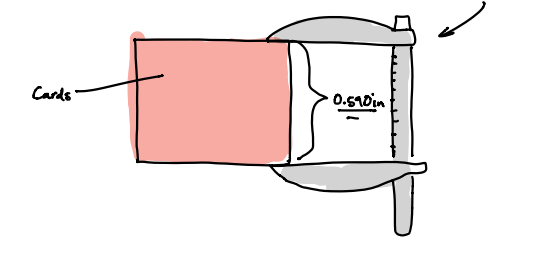
\includegraphics{problem1}
    
    \textbf{Given}
    
    \begin{itemize}
    	\item The measurement tool has an uncertainty of $\pm 0.005$.
    	\item The thickness of 52 cards is 0.590 in.
    \end{itemize}

	\textbf{Find}
	
	\begin{itemize}
		\item The thickness of a single card along with its uncertainty.
		\item The amount of decks must be measured together to find a measurement of a single card with the uncertainty of $0.00002$ in. 
	\end{itemize}

	\textbf{Theory}
	
	\begin{itemize}
	
		\item If $q$ is the quotient of two values ($x$ and $y$) with uncertainties, then $\delta q$ is
		
		\[
			\delta q = |q| \sqrt{(\frac{\delta x}{x})^{2} + (\frac{\delta y}{y})^{2}}	
		\]
		
		\item The thickness, $t$, of a single card can be found with this equation, with T being the thickness of the deck and $N$ being the number of cards
		
		\[
			t = \frac{T}{N}	
		\]
		
		\item When calculating the uncertainty while multiplying by an exact number, simply multiply the uncertainty by the number as shown below
		
		\[
			\delta q = |N| \delta x
		\]
	
	\end{itemize}

	\textbf{Assumptions}
	
	\begin{itemize}
		\item Each card has $\frac{1}{52}$ the thickness of a single deck.
		\item Every deck of cards has the same thickness.
	\end{itemize}
	
	\textbf{Solution A}
	
	\begin{enumerate}
		\item Divide the thickness of the cards by the amount.
		
		\[
		\begin{split}
				q &= \frac{T}{N}
				\\
				&= \frac{0.590}{52}	
				\\
				&= \doubleunderline{0.0113}
		\end{split}
		\] \\
		
		\item Calculate the new uncertainty.
		
		\[
		\begin{split}
			\delta t &= |N| \delta x
			\\
			&= \frac{0.005}{52}
			\\
			&= \doubleunderline{0.0001}
		\end{split}	
		\]
		
		Therefore, the thickness of a single card is $0.0113 \pm 0.0001$ in. \\
	\end{enumerate}
	
	
	\textbf{Solution B} \\
	
	\begin{enumerate}
		\item Take the uncertainty equation that involves exact values and set it up to solve for the number of cards.
		\[
		\begin{split}
			\delta q &= |N| \delta x
			\\
			\frac{\delta q}{\delta x} &= |N|
		\end{split}
		\]
		
		\item Plug in the uncertainty found earlier into the $\delta q$ and plug in the target uncertainty value into $\delta x$.
		\[
		\begin{split}
			\frac{0.0001}{0.00002} &= |N|
			\\
			\doubleunderline{5} &= |N|
		\end{split}
		\]
		
		The amount of cards needed is a factor of 5; therefore, it is logical to assume that 5 decks of cards are needed to reach that uncertainty.
	\end{enumerate}

	\textbf{Conclusion}
	
	Based on the calculations above, the thickness of a single card is 0.0113 inches with an uncertainty of 0.0001 inches, and the amount of decks needed to decreased that uncertainty to 0.00002 is about 5.

\end{homeworkProblem}

\begin{homeworkProblem}
	In an experiment on the conservation of angular momentum, a student needs to find the angular momentum $L$ of a uniform disk of mass $M$ and a radius R as it rotates with angular velocity $\omega$. She makes the following measurements.
	
	\[
	\begin{split}
		M = 1.10 \pm 0.01 \unit{kg}
		\\
		R = 0.250 \pm 0.005 \unit{m}
		\\
		\omega = 2.15 \pm 0.4 \unit{rad/s}
	\end{split}
	\]
	
	and calculates $L$ using $L = \frac{1}{2}MR^{2}\omega$. What is her answer for $L$ with its uncertainty?
	\\
	\\
	\textbf{Diagram}
	
	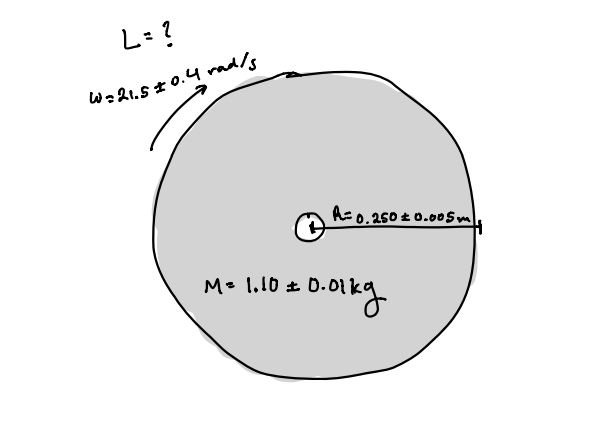
\includegraphics{problem2}
	
	\textbf{Given}
	
	\begin{itemize}
		\item $M = 1.10 \pm 0.01 \unit{kg}$
		\item $R = 0.25 \pm 0.005 \unit{m}$
		\item $\omega = 21.5 \pm 0.4 \unit{rad/s}$
	\end{itemize}

	\textbf{Find}
	
	\begin{itemize}
		\item The angular momentum, $L$, along with its uncertainty.
		\\
		\\
	\end{itemize}

	\textbf{Theory}
	
	\begin{itemize}
		\item The equation for angular momentum is described as:
		\[
			L = \frac{1}{2}MR^{2} \omega
		\]
		\item The equations needed to find uncertainty in this case is:
		\[
		\begin{split}
			\frac{\delta L}{|L|} &= \sqrt{(\frac{0}{0.5})^{2} + (\frac{\omega M}{M})^{2} + (\frac{\omega R}{R})^{2} + (\frac{\delta \omega}{\omega})^{2}}
			\\
			\frac{\delta R^{2}}{|R^{2}|} &= \sqrt{(\frac{\omega R}{R})^{2} + (\frac{\omega R}{R}^{2})}
		\end{split}
		\]
	\end{itemize}

	\textbf{Assumptions}
	
	\begin{itemize}
		\item The angular velocity is constant.
		\item There is no friction.
	\end{itemize}
	
	\textbf{Solution}
	
	\begin{enumerate}
		\item To find angular momentum, $L$, plug in mass, radius, and angular velocity.
		
		\[
		\begin{split}
			L &= \frac{1}{2}MR^{2} \omega
			\\
			&= \frac{1}{2}(1.10 \unit{kg})(0.250 \unit{m})^{2}(21.5 \unit{s^{-1}})
			\\
			&= \doubleunderline{0.739 \unit{\frac{kg * m^{2}}{s}}}
		\end{split}
		\]
		
		\item To find the uncertainties, $\delta L$, plug in the uncertainties of the other variables.
		\[
		\begin{split}
			\frac{\delta R^{2}}{|R|} &= \sqrt{(\frac{0.005 \unit{m}}{0.250 \unit{m}})^{2} + (\frac{0.005 \unit{m}}{0.250 \unit{m}})^{2}}
			\\
			&= \doubleunderline{0.03 \unit{m}}
			\\
			\frac{\delta L}{|L|} &= \sqrt{(\frac{0}{0.5})^{2} + (\frac{0.01 \unit{kg}}{1.10 \unit{kg}})^{2} + (0.03 \unit{m})^{2} + (\frac{0.4 \unit{\frac{rad}{s}}}{21.5 \unit{\frac{rad}{s}}})^{2}}
			\\
			&= \doubleunderline{0.03 \unit{\frac{kg * m^{2}}{s}}}
		\end{split}
		\]
	\end{enumerate}

	\textbf{Conclusion}
	
	The angular momentum is $0.739 \pm 0.03 \unit{\frac{kg * m^{2}}{s}}$.

\end{homeworkProblem}

\pagebreak

\begin{homeworkProblem}
	According to theory, the period $T$ of a simple pendulum is $T = 2 \pi \sqrt{\frac{L}{g}}$.
	\\
	\\
	a) If $L$ is measured as $L = 1.40 \pm 0.01 \unit{m}$ what is the predicted value of $T$?
	\\
	\\
	b) Would you say that a measured value of $T = 2.39 \pm 0.01$ is consistent with the theoretical prediction of part a.
	\\
	
	\textbf{Diagram}
	
	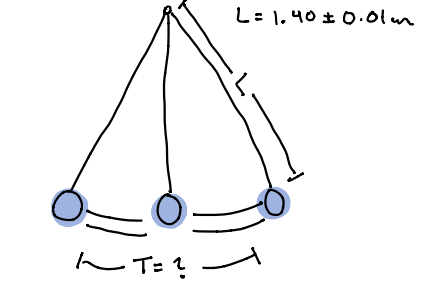
\includegraphics{problem3}
	
	\textbf{Given}
	\begin{itemize}
		\item The length of the pendulum is $1.40 \pm 0.01 \unit{m}$
		\item The measured value of $T = 2.39 \pm 0.01 \unit{s}$ is consistent with the theoretical prediction of part(a).
	\end{itemize}
	
	\textbf{Theory}
	
	\begin{itemize}
		
	
		\item Period can be calculated with the following:
		\[
			T = 2 \pi \sqrt{\frac{L}{g}}
		\]
	\end{itemize}

	\textbf{Assumptions}
	
	\begin{itemize}
		\item All calculations are done with the assumption that the most ideal conditions are present (i.e. lack of air resistance)
		
		\item $g = 9.81 \unit{\frac{m}{s^{2}}}$
	\end{itemize}
	
	\pagebreak
	
	\textbf{Solution A}
	
	\begin{enumerate}
		\item To solve for the period, $T$, plug in the values to the following equation.
		
		\[
		\begin{split}
		T &= 2 \pi \sqrt{\frac{L}{g}}
		\\
		&= 2 \pi \sqrt{\frac{1.40 \unit{m}}{9.81 \unit{\frac{m}{s^{2}}}}}
		\\
		&= 2 \pi (0.378 \unit{s})
		\\
		&= \doubleunderline{2.38 \unit{s}}
		\end{split}		
		\]
		
		\item To find the uncertainty of $T$, take the derivative of and plug the values into the following:
		\[
		\begin{split}
			T &= 2 \pi \sqrt{\frac{L}{g}}
			\\
			\ln T &= 2 \ln( \pi \sqrt{\frac{L}{g}})
			\\
			\ln T &= \ln 2 \pi + \frac{1}{2} \ln L - \frac{1}{2} \ln g
			\\
			\frac{\delta T}{T} (T) &= \frac{\delta L}{2L} (T)
			\\
			\delta T &= \frac{\delta L T}{2 L}
			\\
			&= \frac{(0.01 \unit{m})(2.39 \unit{s})}{2 (1.20 \unit{m})}
			\\
			&= \doubleunderline{0.00854 \unit{s}} 
		\end{split}
		\]
	\end{enumerate}

	\textbf{Solution B}
	
	\begin{itemize}
		\item The measured value yielded nearly the same result but but the calculated value had a greater uncertainty.
	\end{itemize}

	\textbf{Conclusion}
	
	\begin{itemize}
		\item The calculation yielded $2.38 \pm 0.0832 \unit{s}$ which has a smaller uncertainty then the measured value of $2.39 \pm 0.00854 \unit{s}$.
	\end{itemize}
	
\end{homeworkProblem}

\pagebreak

\begin{homeworkProblem}
	To find the acceleration of a glider moving down a sloping air track, you measure its velocity at two points ($v_{1}$ and $v_{2}$) and the time $t$ it takes between them.
	\[
	\begin{split}
		v_{1} = 0.21 \pm 0.05 \unit{\frac{m}{s}}
		\\
		v_{2} = 0.85 \pm 0.05 \unit{\frac{m}{s}}
		\\
		t = 8.0 \pm 0.1 \unit{s}
	\end{split}
	\]
	
	a) Assuming all uncertainties are independent and random, and acceleration is calculated using $a = \frac{v_{2} - v_{1}}{t}$, what should you report for $a$ and its uncertainty?
	\\
	\\
	b) You calculate using an air resistances model that the acceleration should be $0.13 \pm 0.01 \unit{\frac{m}{s^{2}}}$.
	Does your measurement agree with this prediction?
	\\
	\\
	
	\textbf{Diagram}
		
	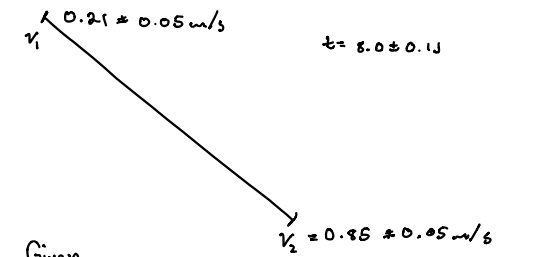
\includegraphics{problem4}
	
	\textbf{Given}
	
		\begin{itemize}
		\item $v_{1} = 0.21 \pm 0.05 \unit{\frac{m}{s}}$
		\item $v_{2} = 0.85 \pm 0.05 \unit{\frac{m}{s}}$
		\item $t = 8.0 \pm 0.1 \unit{s}$
		\end{itemize}
	
	\textbf{Find}
	
	\begin{itemize}
		\item $a$ and its uncertainty.
		\item How does the measurement compare to a calculation of $0.13 \pm 0.01 \unit{m}{s^{2}}$.
	\end{itemize}

	\textbf{Theory}
	
	\begin{itemize}
		\item The equation for acceleration is as follows:
		
		\[
		a = \frac{v_{2} - v_{1}}{t}
		\]
	\end{itemize}

	\textbf{Assumption}
	
	\begin{itemize}
		\item There is no air resistance.
	\end{itemize}
		 
	\textbf{Solution}
	
	\begin{enumerate}
		\item Plug all the variables into the acceleration equation to get acceleration:
		
		\[
		\begin{split}
			a &= \frac{v_{2}-v_{1}}{t}
			\\
			&= \frac{0.85 \unit{\frac{m}{s}} - 0.21 \unit{\frac{m}{s}}}{8.0 \unit{s}}
			\\
			&= \doubleunderline{0.080 \unit{\frac{m}{s^{2}}}}
		\end{split}
		\]
		
		\item To find the uncertainty of $a$, the uncertainty of $\Delta v$ must be found. 
		
		\[
		\begin{split}
			\delta \Delta v &= \sqrt{(0.05 \unit{\frac{m}{s}})^{2} + (0.05 \unit{\frac{m}{s}})^{2}}
			\\
			&= \doubleunderline{0.07071 \unit{\frac{m}{s}}}
		\end{split}
		\]
		
		\item Now, plug in $\delta \Delta V$, $\Delta V$, and $t$ into the equation to get $\delta a$.
		
		\[
		\begin{split}
			\delta a &= 0.080 \sqrt{(\frac{0.07 \unit{\frac{m}{s}}}{0.64 \unit{\frac{m}{s}}})^{2}(\frac{0.1 \unit{\frac{m}{s}}}{8.0 \unit{\frac{m}{s}}})^{2}}
			\\
			&= \doubleunderline{0.01 \unit{\frac{m}{s^{2}}}}
		\end{split}
		\]
		
	\end{enumerate}

	\textbf{Conclusion}
	
	\begin{enumerate}
			\item The calculation yielded $0.080 \pm 0.01 \unit{\frac{m}{s^{2}}}$ therefore the measurement does not agree.
	\end{enumerate}
\end{homeworkProblem}

\pagebreak

\begin{homeworkProblem}
	An Atwood machine consists of two masses $m_{1}$ and $m_{2}$ (with $m_{1} > m_{2}$) attached to the ends ends of a light string that passes over a light, friction-less pulley. When the masses are released, the mass $m_{1}$ is easily shown to accelerate down with an acceleration
	
	\[
		a = g \frac{m_{1} - m_{2}}{m_{1} + m_{2}}
	\] 
	
	Suppose that $m_{1}$ and $m_{2}$ are measured as $m_{1} = 100 \pm 1 \unit{gram}$ and $m_{2} = 50 \pm 1 \unit{gram}$. Derive a formula of the uncertainty in the expected acceleration in terms of the masses and their uncertainties, and the calculate $\delta a$ for the given numbers.
	\\
	\\
	
	\textbf{Diagram}
	
	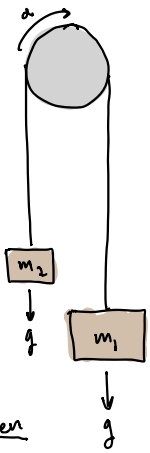
\includegraphics{problem5}
	
	\textbf{Given}
	
	\begin{itemize}
		\item $m_{1} = 100 \pm 1 \unit{gram}$
		\item $m_{2} = 50 \pm 1 \unit{gram}$
	\end{itemize}

	\textbf{Find}
	
	\begin{itemize}
		\item Derive a formula of uncertainty that gives an expected acceleration in terms of the masses and their uncertainties.
		\item Calculate $\delta a$.
	\end{itemize}

	\textbf{Theory}
	
	\begin{itemize}
		\item This equation shows how the masses are related to find acceleration.
		
		\[
			a = g \frac{m_{1} - m_{2}}{m_{1} + m_{2}}
		\]
	\end{itemize}

	\textbf{Assumption}
	
	\begin{enumerate}
		\item Plug in variables to calculate $a$. 
		
		\[
		\begin{split}
			a &= g \frac{m_{1} - m_{2}}{m_{1} + m_{2}}
			\\
			&= (9.81 \unit{\frac{m}{s^{2}}}) \frac{100 \unit{g} - 50 \unit{g}}{100 \unit{g} + 50 \unit{g}}
			\\
			&= \doubleunderline{3.27 \unit{\frac{m}{s^{2}}}}
		\end{split}
		\]
		
		\item To calculate the uncertainty, the following equation needs to be derived.
		
		\[
		\begin{split}
			\ln a &= \ln{g \frac{m_{1} - m_{2}}{m_{1} + m_{2}}} 
			\\
			&= \ln g + \ln(m_{1} - m_{2}) - \ln(m_{1} + m_{2})
		\end{split}
		\]
		
		\item Take the derivative.
		
		\[
		\begin{split}
			\frac{\delta a}{a} &= \frac{\delta m_{1} - \delta m_{2}}{m_{1} - m_{2}} - \frac{\delta m_{1} + \delta m_{2}}{m_{1} + m_{2}}
			\\
			\delta a &= a (\frac{\delta m_{1} - \delta m_{2}}{m_{1} - m_{2}} - \frac{\delta m_{1} + \delta m_{2}}{m_{1} + m_{2}})
		\end{split}
		\]
		
		\item Plug everything in. 
		
		\[
		\begin{split}
			\delta &= (\frac{0 \unit{g}}{50 \unit{g}} - \frac{2 \unit{g}}{150 \unit{g}})(3.27 \unit{m}{s^{2}})
			\\
			&= \doubleunderline{0.044 \unit{\frac{m}{s^{2}}}}
		\end{split}
		\]
		
	\end{enumerate}

	\textbf{Conclusion}
	
	\begin{enumerate}
		\item The acceleration of the system is $3.27 \pm 0.044 \unit{\frac{m}{s^{2}}}$.
		\item The following equation was derived to reach that uncertainty:
		
		\[
				\frac{\delta a}{a} = \frac{\delta m_{1} - \delta m_{2}}{m_{1} - m_{2}} - \frac{\delta m_{1} + \delta m_{2}}{m_{1} + m_{2}}
		\]
	\end{enumerate}
\end{homeworkProblem}

\end{document}
